\section{Metodología}
\label{sec:met}

\subsection{Plataforma experimental}
La Tabla~\ref{tab:hw} resume el hardware. Se adopta la convención de las notas: sistema del cuerpo $\{B\}$ con $x$ hacia adelante, $y$ hacia la derecha y $z$ hacia abajo, ángulos de Euler $ZYX$ y rotores numerados 1 a 4 (adelante-izquierda, adelante-derecha, atrás-derecha, atrás-izquierda) en $\bm r_1=(l,-l,0)$, $\bm r_2=(l,l,0)$, $\bm r_3=(-l,l,0)$, $\bm r_4=(-l,-l,0)$. El dron no tiene medición de tensión de batería ni de posición lateral; esto limita el análisis (Sección~\ref{sec:disc}).

\begin{table}[t]
\caption{Componentes de la plataforma.}
\label{tab:hw}
\centering\small
\begin{tabular}{@{}lp{5.7cm}@{}}
\toprule
Elemento & Descripción \\
\midrule
Marco y propulsión & F450; 4 $\times$ A2212 1000\,KV; hélice APC 10$\times$4.5\,MR \\
Actuación & 4 ESC 30\,A, PWM a 50\,Hz, recorrido 1040--1800\,\textmu{}s \\
Controlador & ESP32-S3 (núcleo 1: control a 250\,Hz; núcleo 0: sensores y web) \\
Actitud & MPU-6500 (I$^2$C), filtro de Mahony \\
Altura & VL53L0X (ToF, útil $<$25\,cm), HC-SR04 (útil 8\,cm--3.5\,m) \\
Enlace & Punto de acceso WiFi y página de control, caja negra a 50\,Hz \\
\bottomrule
\end{tabular}
\end{table}

\subsection{Modelo dinámico}
Se usa el modelo de las notas~\cite{notas1}. Con $\bm\eta=(\phi,\theta,\psi)$ y $\bm\omega=(p,q,r)$ en $\{B\}$, la cinemática de Euler es
\begin{align}
\dot\phi&=p+q\sin\phi\tan\theta+r\cos\phi\tan\theta,\nonumber\\
\dot\theta&=q\cos\phi-r\sin\phi,\label{eq:euler}\\
\dot\psi&=(q\sin\phi+r\cos\phi)/\cos\theta,\nonumber
\end{align}
la traslación, con $u_1=-f_t/m$, es $\ddot x=r_{13}u_1$, $\ddot y=r_{23}u_1$, $\ddot z=g+r_{33}u_1$ con $r_{33}=\cos\theta\cos\phi$, y la rotación es $I\dot{\bm\omega}+\bm\omega\times(I\bm\omega)=\btau$ con $I=\mathrm{diag}(I_x,I_y,I_z)$. Cada rotor produce $f_i=k_f\omega_i^2$ y $\tau_i=k_m\omega_i^2$, de modo que
\begin{equation}
\begin{bmatrix}f_t\\ \tau_x\\ \tau_y\\ \tau_z\end{bmatrix}=
\begin{bmatrix}
k_f&k_f&k_f&k_f\\
k_fl&-k_fl&-k_fl&k_fl\\
k_fl&k_fl&-k_fl&-k_fl\\
k_m&-k_m&k_m&-k_m
\end{bmatrix}
\begin{bmatrix}\omega_1^2\\ \omega_2^2\\ \omega_3^2\\ \omega_4^2\end{bmatrix}.
\label{eq:mezcla}
\end{equation}
Con $\omega_{\min}=0.15\,\omega_{\max}$ y $\omega_{\max}=1046$\,rad/s (estimada a partir de $KV\cdot V_{bat}\cdot\eta$, único parámetro del mapeo que no se midió), el conjunto factible es el politopo $\omega_{\min}^2\le\omega_i^2\le\omega_{\max}^2$.

\subsection{Identificación de parámetros}
\label{sec:ident}
Los parámetros se obtuvieron con tres ensayos (hoja de cálculo del proyecto).

\textbf{Masa y brazo.} La masa en vuelo es $m=1.0022$\,kg. El brazo efectivo es $l=0.1616$\,m, es decir, la distancia centro--motor ($0.2285$\,m) proyectada sobre los ejes $x$ e $y$ ($l=L/\sqrt2$).

\textbf{Inercias (péndulo bifilar).} El dron se cuelga de dos hilos de longitud $L_h$, cada uno a una distancia $R$ del eje a medir (separación $2R$), y se miden cinco ensayos de cinco oscilaciones. Para un péndulo bifilar~\cite{jardin}, $T=2\pi\sqrt{I L_h/(mgR^2)}$, de donde
\begin{equation}
I=\frac{m\,g\,R^2\,T^2}{4\pi^2 L_h}.
\label{eq:bifilar}
\end{equation}
Los pares $(R,L_h)$ son $(0.047,0.53)$, $(0.0525,0.34)$ y $(0.06,0.88)$\,m para los ejes $x$, $y$ y $z$. La incertidumbre combina la dispersión de los periodos, la resolución del cronómetro y las de la balanza y la cinta métrica; el montaje, las mediciones y la propagación completa están en el Anexo~A.

\textbf{Empuje y par.} Se midió el empuje de un motor con hélice para pulsos de 1000 a 1750\,\textmu{}s (16 puntos, en gramos-fuerza). El empuje sigue $F=K_f(\mathrm{PWM}-\mathrm{PWM}_0)^2+c'$, con $\mathrm{PWM}_0=-b/2a$ y $c'=c-b^2/4a$ obtenidos de un ajuste cuadrático $F=a\,\mathrm{PWM}^2+b\,\mathrm{PWM}+c$ sobre los puntos no atípicos (se descartan 1450, 1500 y 1550\,\textmu{}s); luego $K_f$ sale de una regresión lineal de $F-c'$ contra $(\mathrm{PWM}-\mathrm{PWM}_0)^2$ (la hoja usa en esta regresión los puntos de 1000 a 1500\,\textmu{}s). El coeficiente de par se obtiene sin medir torque, con la relación entre empuje y par de la hélice, $k_m=\alpha^2k_f$, $\alpha^2=C_P D/(2\pi C_T)$, con $C_T=0.1125$, $C_P=0.0441$ y $D=0.254$\,m de la hélice APC 10$\times$4.5\,MR.

\textbf{Unidades del firmware.} El mezclador necesita $k_f$ en N/(rad/s)$^2$. Se fija $k_f=3.2107\times10^{-6}$ de modo que $4k_f\omega_{\max}^2=14.05$\,N, y $k_m=\alpha^2k_f=5.088\times10^{-8}$. La relación $k_fl/k_m=10.2$ determina el reparto del mezclador (Sección~\ref{sec:control}).

\subsection{Arquitectura de control}
\label{sec:control}
La Fig.~\ref{fig:arq} muestra la arquitectura; las ecuaciones citadas son las de las notas~\cite{notas1}.

\begin{figure*}[t]
\centering
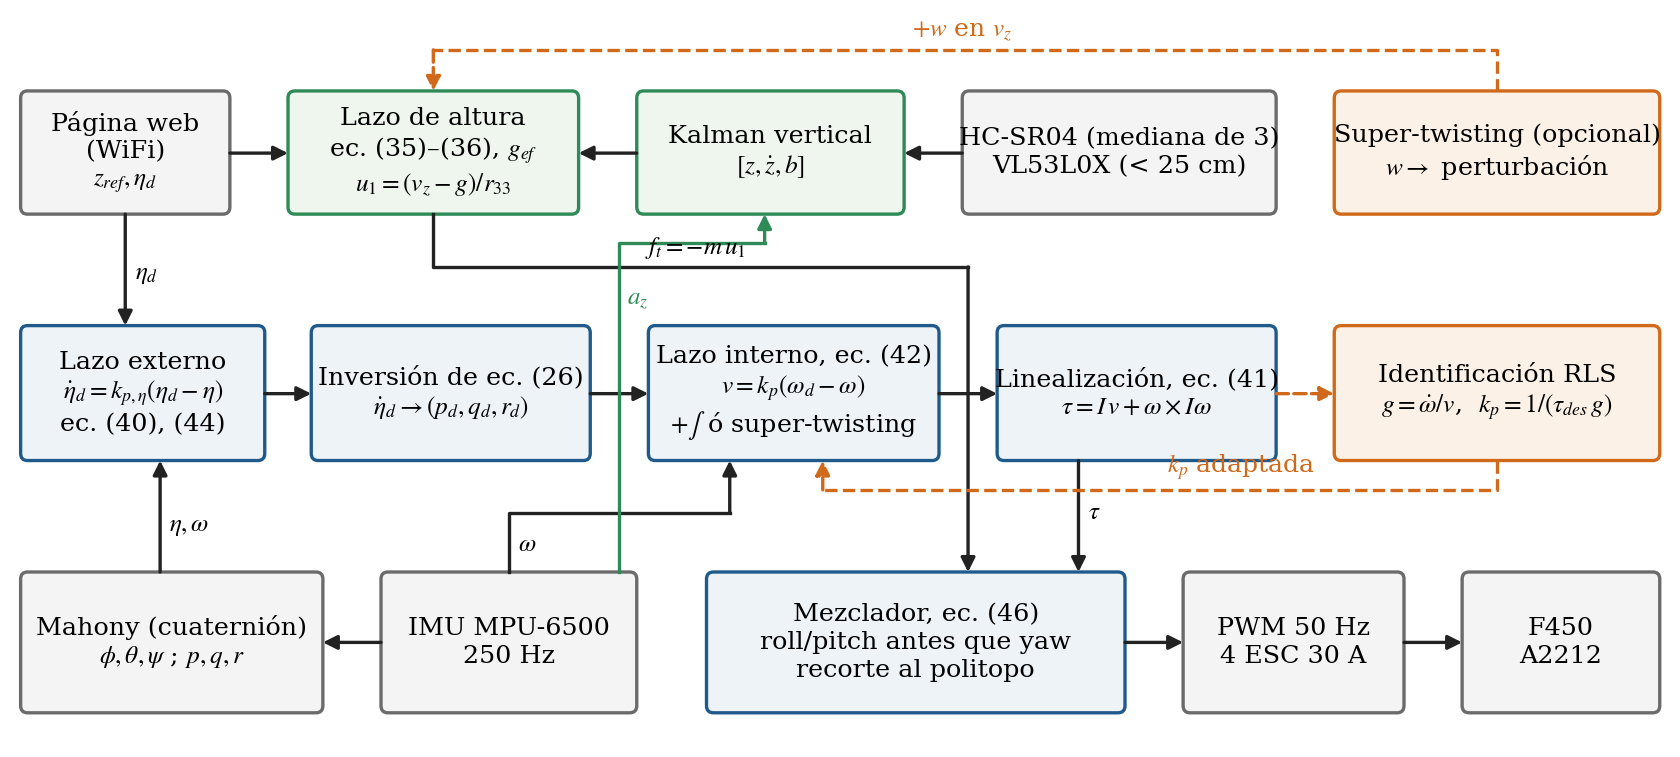
\includegraphics[width=0.93\textwidth]{f_arquitectura.png}
\caption{Arquitectura de control del firmware V\_11. En verde, el lazo de altura y su estimador; en azul, la cascada de actitud; en naranja, las extensiones robusta y adaptativa; en gris, sensores y actuadores.}
\label{fig:arq}
\end{figure*}

\textbf{Altura (ec. 35--36).} Con $v_z=\ddot z_d-k_{d,z}(\dot z-\dot z_d)-k_{p,z}(z-z_d)$ se impone $\ddot e_z+k_{d,z}\dot e_z+k_{p,z}e_z=0$ mediante
\begin{equation}
u_1=\frac{v_z-g_{ef}}{r_{33}},\qquad f_t=-m\,u_1,
\label{eq:altura}
\end{equation}
donde $g_{ef}$ es la prealimentación de hover: se carga al entrar en el modo MANTENER con el empuje que el dron está dando en ese instante ($g_{ef}=f_t r_{33}/m$, acotada a $[0.55,1.35]\,g$), en lugar de $g$ del modelo. Se añade un integrador ($k_{i,z}=1$, tope 2\,m/s$^2$, con anti-windup) y el empuje se acota a $[0.45,1.35]$ veces el de hover. Con $k_{p,z}=4$ y $k_{d,z}=3.6$ se tiene $\omega_n=2$\,rad/s y $\zeta=0.9$.

\textbf{Actitud.} El lazo externo impone $\dot\phi_d=k_{p,\phi}(\phi_d-\phi)$ (ec. 40; igual para $\theta$ y, con ec. 44, para $\psi$) y las velocidades deseadas del cuerpo salen de invertir (\ref{eq:euler}):
\begin{align}
p_d&=\dot\phi_d-\dot\psi_d\sin\theta,\nonumber\\
q_d&=\dot\theta_d\cos\phi+\dot\psi_d\cos\theta\sin\phi,\label{eq:inv}\\
r_d&=-\dot\theta_d\sin\phi+\dot\psi_d\cos\theta\cos\phi.\nonumber
\end{align}
El lazo interno es $v_p=k_{p,p}(p_d-p)$ (ec. 42, igual para $q$ y $r$) y el torque sale de la linealización (ec. 41)
\begin{align}
u_x&=I_xv_p+(I_z-I_y)qr,\nonumber\\
u_y&=I_yv_q+(I_x-I_z)pr,\label{eq:lin}\\
u_z&=I_zv_r+(I_y-I_x)pq.\nonumber
\end{align}
La Tabla~\ref{tab:gan} lista las ganancias por defecto. Con $k_{p,p}=15$\,s$^{-1}$ el lazo interno tiene constante de tiempo de $67$\,ms y con $k_{p,\phi}=6$\,s$^{-1}$ el externo, $167$\,ms, es decir, 2.5 veces más lento, como exige una cascada. El integrador de velocidad angular ($k_i$) viene en cero: primero se sintoniza el proporcional puro de las notas.

\begin{table}[t]
\caption{Ganancias y límites por defecto (\texttt{config.h}).}
\label{tab:gan}
\centering\small
\begin{tabular}{@{}lcc@{}}
\toprule
Lazo & Roll / Pitch & Yaw \\
\midrule
Ángulo $k_{p,\eta}$ [s$^{-1}$] & 6.0 & 2.5 \\
Velocidad angular $k_{p,\omega}$ [s$^{-1}$] & 15 & 5 \\
Super-twisting $(k_1,k_2)$ [rotación] & (3, 8) & (2, 5) \\
Altura $(k_{p,z},k_{d,z},k_{i,z})$ & \multicolumn{2}{c}{(4, 3.6, 1)} \\
Super-twisting altura $(k_1,k_2)$ & \multicolumn{2}{c}{(1.5, 2)} \\
Referencia máx. / corte de seguridad & \multicolumn{2}{c}{$25^\circ$ / $60^\circ$} \\
\bottomrule
\end{tabular}
\end{table}

\textbf{Mezclador con prioridad de ejes.} La inversa de (\ref{eq:mezcla}) da $\omega_i^2$. Como $k_fl/k_m=10.2$, un N\,m de yaw cuesta diez veces más rango de motor que uno de roll. Una caja negra previa mostró que el 94\,\% del rango de motor se gastaba en yaw y que el mezclador estaba saturado el 93\,\% del tiempo. Por ello V\_9 reparte por prioridad: primero el empuje, luego roll y pitch con todo el rango que necesiten (factor $s_{rp}\in[0,1]$) y el yaw con lo que sobre, nunca más del 30\,\% del recorrido. Sustituye al recorte componente a componente de las notas, que cambia la dirección del torque.

\textbf{Extensión robusta (super-twisting).} Tras la linealización cada lazo es $\dot s=v+d(t)$ con $d$ la incertidumbre del modelo. Con la superficie $s$ (error de velocidad angular, o $\sigma=\lambda(z_d-z)-\dot z$ en altura) se añade
\begin{equation}
v=k_1|s|^{1/2}\mathrm{sat}(s/\varphi)+w,\qquad \dot w=k_2\,\mathrm{sat}(s/\varphi),
\label{eq:st}
\end{equation}
que es el algoritmo de Levant~\cite{levant}, continuo, converge en tiempo finito si $k_2>L$ y $k_1>1.5\sqrt L$ con $|\dot d|\le L$, y cuyo estado $w$ estima $-d$. Se usa una capa límite $\varphi$ (0.10\,rad/s) para evitar el \emph{chattering} con el giroscopio ruidoso y el integrador se anula mientras está activo. Es la contraparte, en este dron, del SMC del bloque de control robusto del curso~\cite{notas2}.

\textbf{Extensión adaptativa (identificación recursiva).} Tras (\ref{eq:lin}) cada eje cumple $\dot\omega=g\,v$ con $g=1$ si el modelo es exacto. Se estima $g$ por mínimos cuadrados recursivos con olvido $\lambda=0.999$, aplicando el \emph{mismo} filtro de 8\,Hz a $\dot\omega$ y a $v$ (para que el desfase se cancele) y aprendiendo solo con excitación suficiente y sin saturación. Con $g$ se fija el ancho de banda y no la ganancia: $k_p=1/(\tau_{des}\,\hat g)$. Un $\hat g<0$ diagnostica un signo invertido.

\subsection{Estimación de estado}
\textbf{Actitud.} Filtro de Mahony~\cite{mahony} sobre cuaternión ($K_p=2$, $K_i=0.05$); la corrección solo se aplica si $0.5<|\bm a|<1.6$\,g. Sin magnetómetro el yaw deriva.

\textbf{Altura.} Filtro de Kalman~\cite{kalman} de tres estados $\bm x=[z,\dot z,b]^\top$ (z positivo hacia abajo, $b$ sesgo del acelerómetro). La predicción usa la aceleración vertical inercial $a_v=r_{31}a_x+r_{32}a_y+r_{33}a_z+g$ como entrada, y la corrección usa la distancia al suelo corregida por $r_{33}$. Manda el ultrasonido (mediana de 3 ecos), y el ToF solo bajo 25\,cm, con histéresis de 5\,cm en la frontera. La V\_11 re-sintoniza el filtro con el ruido medido en vuelo: $\sigma_{US}=0.05+0.08\,d$ (m), puerta de innovación de $4\sigma$, reanclaje tras 3 rechazos seguidos, $a_v$ filtrada a 20\,Hz y acotada a $\pm6$\,m/s$^2$, ruido de proceso mínimo de 3\,(m/s$^2$)$^2$ y deriva del sesgo $0.2$\,(m/s$^2$)$^2$/s. La medida de distancia se acepta solo entre 8\,cm y 3.5\,m (ultrasonido).

\subsection{Implementación, seguridad y desarrollo iterativo}
El lazo de control corre a 250\,Hz en el núcleo 1; los sensores a 20\,Hz y el servidor web en el núcleo 0. El PWM es de 50\,Hz, lo que impone un retardo de actuación de hasta 20\,ms y limita la ganancia útil del lazo interno. El arranque exige empuje 0 y dron casi nivelado; hay desarme a $60^\circ$ o si la IMU calla 100\,ms, y bajada automática si el enlace calla 0.8\,s.

El firmware se refinó en ciclos de vuelo--análisis--corrección (Tabla~\ref{tab:vers}); cada cambio responde a un hallazgo de una caja negra.

\begin{table}[t]
\caption{Evolución del firmware y su motivo.}
\label{tab:vers}
\centering\small
\begin{tabular}{@{}lp{6.1cm}@{}}
\toprule
Versión & Cambio y motivo \\
\midrule
V\_8 & Referencia de altura fija, nivel fino, página reducida. \\
V\_9 & Prioridad roll/pitch sobre yaw en el mezclador (94\,\% del rango en yaw). \\
V\_10 & Filtro del acelerómetro, solo medidas nuevas y crudas, rechazo de rebotes, hover aprendido; V\_10b: reanclaje del filtro porque la altura estimada divergía. \\
V\_11 & Kalman con el ruido medido del ultrasonido (13\,cm a 1.2\,m, no 4\,cm), mediana de ecos, $a_z$ filtrada y acotada, CSV sin duplicados. \\
\bottomrule
\end{tabular}
\end{table}

\subsection{Protocolo experimental y procesamiento}
La caja negra graba a 50\,Hz al armar y se descarga en CSV de 25 columnas: tiempo, modo, estado del mezclador, ángulos, velocidades angulares, altura estimada y de referencia, velocidad vertical, empuje, ambos sensores de distancia, mando por motor y aceleración vertical. Todos los vuelos son del 26-nov-2026. Se analizan los registros recortados a los tramos de interés (los huecos se detectan por saltos de tiempo $>0.1$\,s y no se unen): dos vuelos V\_11 (A: 19:09:36, 21.0\,s; B: 19:25:45, 33.0\,s) y cinco de V\_10/V\_10b como referencia. Las métricas se calculan sobre las muestras con altura estimada $>0.15$\,m (``en el aire''), con el script \texttt{make\_figures.py}. Las ganancias son las por defecto de la Tabla~\ref{tab:gan}. El CSV no registra la referencia de actitud ni los interruptores robusto/adaptativo, que por defecto están apagados, ni la tensión de batería.
